\documentclass[12pt]{article}
\usepackage[utf8]{inputenc}
\usepackage[T1]{fontenc}
\usepackage[spanish,es-tabla]{babel}
\usepackage[left=1.54cm,right=1.54cm,top=1.5cm,bottom=1.8cm]{geometry}
\usepackage{amsmath,amssymb}
\usepackage{graphicx}
\usepackage{enumitem}
\usepackage{booktabs}
\usepackage{tikz}

\pagestyle{plain}
\setlength{\parindent}{0pt}
\setlength{\parskip}{0.4em}

\begin{document}
\shorthandoff{<>}
\large

% ---------- Encabezado ----------
\noindent
\begin{minipage}[t]{0.45\textwidth}
\raggedright
Mec\'anica de Fluidos CI3162\\
Primavera 2026
\end{minipage}%
\hfill
\begin{minipage}[t]{0.45\textwidth}
\raggedleft
Prof.\ Alberto de la Fuente Stranger\\
Auxs.\hspace{0.6cm}Josefina Moreno Faune\\
Sebasti\'an Fredes Ojeda
\end{minipage}

\vspace{3pt}
\hrule
\vspace{-5pt}

\begin{center}
{\Huge\bfseries Clase Auxiliar C1}\\[6pt]
Viernes 4 de Septiembre 2026
\end{center}

\vspace{20pt}

% ======================================================================
\noindent{\LARGE\bfseries Problema 1}
\vspace{6pt}

\noindent Considere un carro de masa $M$ que se encuentra sobre ruedas y que puede
desplazarse libremente por un plano inclinado en un \'angulo $\alpha$, salvo porque el
carro est\'a amarrado a una cuerda que, en el inicio del plano inclinado, est\'a
enrollada en un cilindro de radio $R_e$ y alto $H$. Al interior de este cilindro se
encuentra otro cilindro de radio $R_i$ que est\'a en reposo. Entre ambos cilindros se
encuentra un l\'iquido lubricante de viscosidad $\mu$ (ver Figura 1).

\begin{enumerate}[label=\alph*)]
\item Considerando que el carro se mueve con velocidad $U$ constante, encuentre una
relaci\'on algebraica para calcular $U$ en funci\'on del resto de los par\'ametros del
problema.
\item Determine el valor de $R_i$ necesario para que la velocidad m\'axima a la cual
cae el carro sea igual a la indicada en la Tabla 1.
\end{enumerate}

\begin{center}
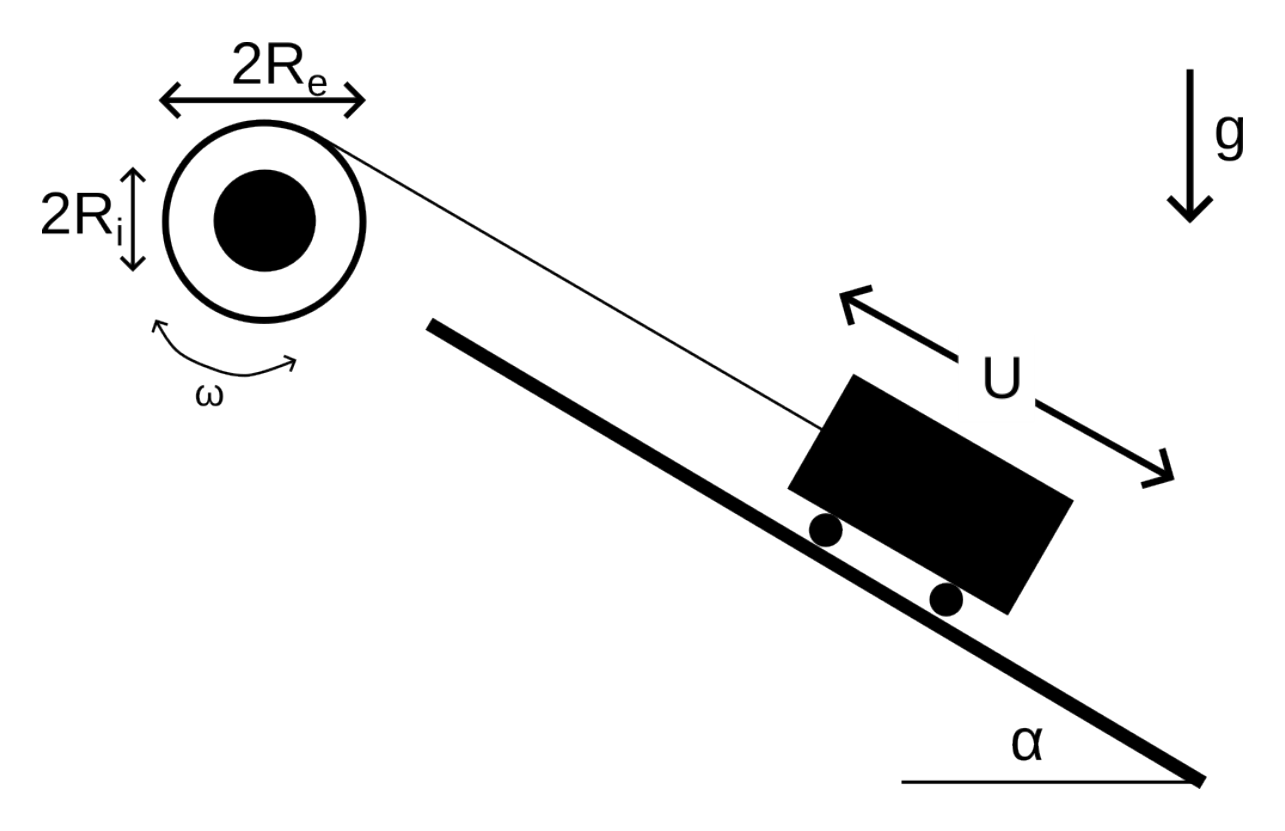
\includegraphics[width=0.5\linewidth]{figs/figura2_P3.png}\\[2pt]
{\normalsize Figura 1}
\end{center}

\begin{center}
{\normalsize Tabla 1: Valores para evaluaci\'on num\'erica}\\[4pt]
\begin{tabular}{@{}lccccccc@{}}
\toprule
$H$ [cm] & $R_e$ [cm] & $\nu$ [cSt] & $\rho_{aceite}$ [gr/cm$^3$] & $M$ [kg] & $U$ [m/s] & $\alpha$ [$^\circ$] \\
\midrule
50 & 15 & 70 & 0{,}9 & 6{,}0 & 1 & 30 \\
\bottomrule
\end{tabular}
\end{center}

\newpage
% ======================================================================
\noindent{\LARGE\bfseries Problema 2}
\vspace{6pt}

\noindent Considere dos recipientes que est\'an separados por una compuerta plana
circular de di\'ametro $D$, inclinada en un \'angulo $\theta$ y rotulada en su extremo
m\'as alto. En el lado izquierdo de la compuerta, el agua se encuentra a una altura
$H_1$ respecto de la r\'otula, mientras que en el lado derecho el recipiente est\'a
tapado pero cuenta con un tubo donde el agua alcanza una altura $\Delta H$ respecto del
nivel de agua del lado izquierdo. En el extremo m\'as sumergido de la compuerta existe
un tope que puede resistir una fuerza m\'axima $F_{max}$ (ver Figura 2).

\begin{enumerate}[label=\alph*)]
\item Calcule la resultante de fuerzas y el torque de presi\'on que ejerce el agua del
lado izquierdo de la compuerta sobre \'esta.
\item Calcule el valor de $F_{max}$ para el valor de $\Delta H$ indicado en la Tabla 2.
\end{enumerate}

\begin{center}
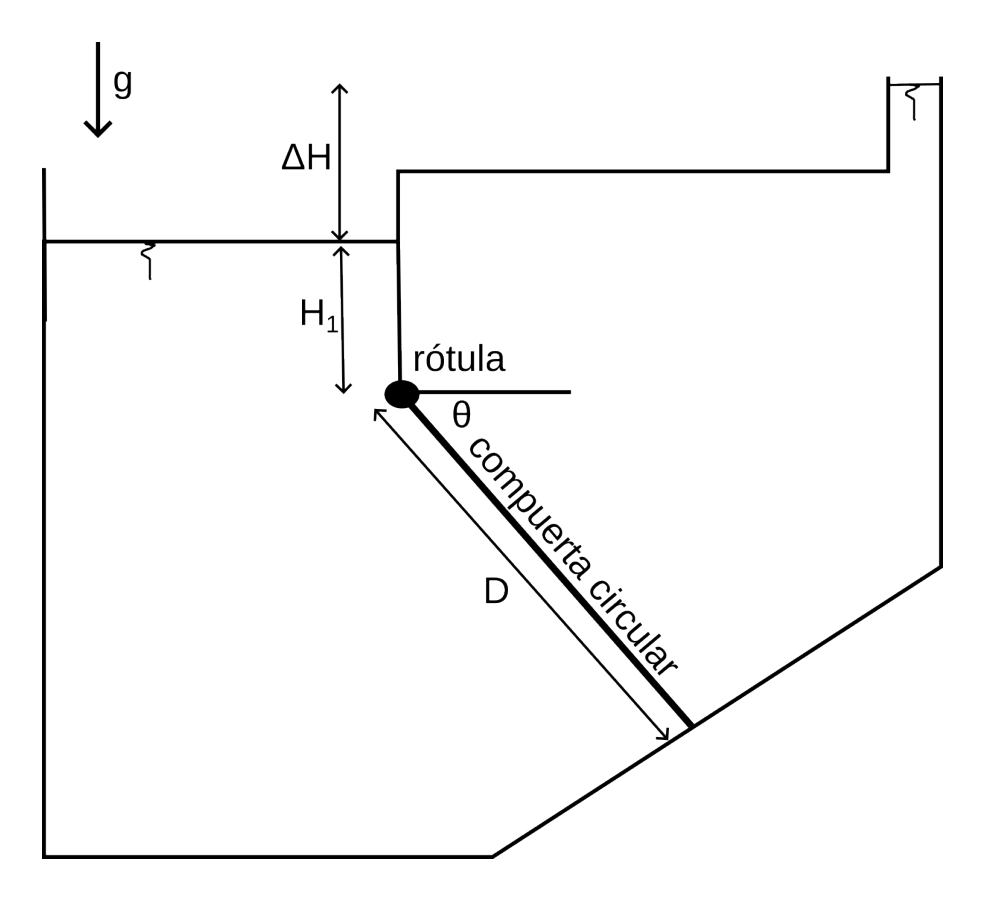
\includegraphics[width=0.38\linewidth]{figs/figura3_P4.png}\\[2pt]
{\normalsize Figura 2}
\end{center}

\begin{center}
{\normalsize Tabla 2: Valores para evaluaci\'on num\'erica}\\[4pt]
\begin{tabular}{@{}lcccc@{}}
\toprule
$D$ [m] & $\theta$ [$^\circ$] & $H_1$ [m] & $\Delta H$ [m] \\
\midrule
2{,}5 & 40 & 0{,}5 & 0{,}6 \\
\bottomrule
\end{tabular}
\end{center}

\newpage
% ======================================================================
\noindent{\LARGE\bfseries Problema 3}
\vspace{6pt}

\noindent Se tiene un cilindro de di\'ametro $D$ que, en su extremo inferior, est\'a
tapado por una compuerta esf\'erica rotulada en el di\'ametro. El cilindro tiene una
altura $H$ y se llena, en primer lugar, con un l\'iquido de densidad $\rho_1$ hasta la
altura $H/3$; luego se llena hasta $2H/3$ con un l\'iquido de densidad $\rho_2 < \rho_1$;
finalmente se tapa de modo que el aire en el \'ultimo tercio queda a presi\'on $P_g$. El
aire fuera del cilindro se encuentra a presi\'on atmosf\'erica (ver Figura 3).

\begin{enumerate}[label=\alph*)]
\item Calcule la presi\'on del l\'iquido en el punto m\'as alto de la compuerta
esf\'erica.
\item Calcule la fuerza de presi\'on que debe resistir la r\'otula.
\end{enumerate}

\begin{center}
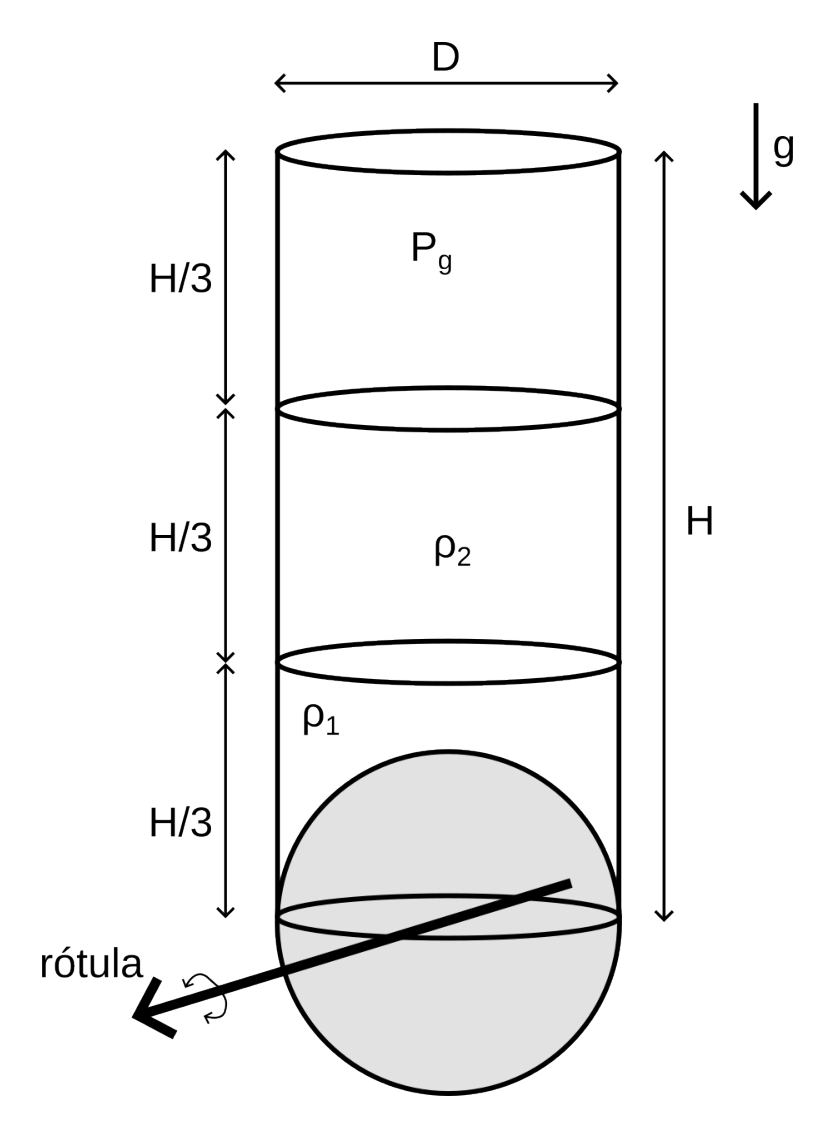
\includegraphics[width=0.3\linewidth]{figs/figura4_P5.png}\\[2pt]
{\normalsize Figura 3}
\end{center}

\begin{center}
{\normalsize Tabla 3: Valores para evaluaci\'on num\'erica}\\[4pt]
\begin{tabular}{@{}lccccc@{}}
\toprule
$H$ [cm] & $D$ [cm] & $\rho_1$ [kg/m$^3$] & $\rho_2$ [kg/m$^3$] & $P_g$ [Atm] \\
\midrule
60 & 2 & 1030 & 1000 & 0{,}9 \\
\bottomrule
\end{tabular}
\end{center}


\newpage
% ======================================================================
\noindent{\LARGE\bfseries Problema 4}
\vspace{6pt}

\noindent Determine la presi\'on y la fuerza del gas en el sistema de la Figura 4 para
que se abra la compuerta semicil\'indrica articulada en $O$. Considerar ancho $L$
perpendicular a la hoja y que el peso de la compuerta es despreciable.

\begin{center}
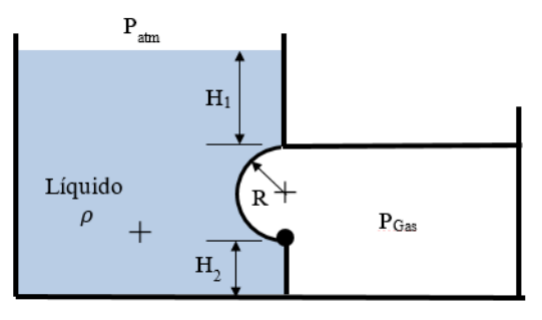
\includegraphics[width=0.5\linewidth]{figs/figura4_P4_original.png}
\end{center}
\begin{center}
{\normalsize Figura 4: Esquema del problema.}
\end{center}

\end{document}
